\section{Ejercicio 3}
\subsection{Introducci\'on}
\noindent
En este ejercicio se plantea la implementaci\'on de la tabla de verdad propuesta por la consigna, la misma se puede ver en la tabla \ref{ej3_tabla_de_verdad}. Para ello se hará uso de compuertas lógicas de tecnología CMOS dispuestas en una placa PCB, con la intención de realizar mediciones relevantes de la configuración de menor costo, con la finalidad de proponer cambios de ser necesarios para evitar posibles problemas con dicha implementación. 
%
\subsection{An\'alisis Te\'orico}
\noindent
De esta manera se hallar\'a el circuito que se realizar\'a mediante las simplificaciones del diagrama de Karnaugh haciendo uso de la tabla propuesta. De esta manera en la imagen siguiente se procede a mostrar dicho diagrama seleccionando los grupos de inter\'es que generan la configuraci\'on de menor costo.
%
\begin{table}[H]
\caption{Tabla propuesta}
\label{ej3_tabla_de_verdad}
\centering
\begin{tabular}{|l|l|l||l|}
\hline
A & B & C & Y \\ \hline \hline
0 & 0 & 0 & 0 \\ \hline
0 & 0 & 1 & 1 \\ \hline
0 & 1 & 0 & 1 \\ \hline
0 & 1 & 1 & 1 \\ \hline
1 & 0 & 0 & 0 \\ \hline
1 & 0 & 1 & 1 \\ \hline
1 & 1 & 0 & 0 \\ \hline
1 & 1 & 1 & 0 \\ \hline
\end{tabular}
\end{table}
%
\begin{center}
    \begin{Karnaughvuit}
       \minterms{1,4,5,6}
        \maxterms{0,2,3,7}
       %\indeterminats{2,5}
       \implicantcostats{4}{6}{green}
       \implicant{1}{5}{blue}
    \end{Karnaughvuit}
\end{center}
%
%
%
\noindent
Así la configuraci\'on l\'ogica que cumple este circuito es la de la ecuaci\'on \ref{ej3_eq1}.
%
\begin{equation}
    \overline{A} \cdot B+\overline{B} \cdot C
    \label{ej3_eq1}
\end{equation}
%
\noindent
Dicha ecuación representa la configuración lógica de menor costo que cumple con la tabla propuesta (tabla \ref{ej3_tabla_de_verdad}).\\
\noindent
De esta forma el circuito que cumple con dicha ecuación se muestra en la figura \ref{ej3_circuito}.
%
\begin{figure}[H]
    \centering
        \centering
        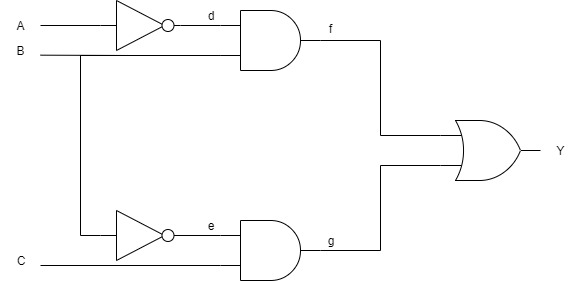
\includegraphics[width=0.8\textwidth]{figs/Ej3/circuito1.jpg} % first figure itself
         \caption{Figura del circuito con la configuraci\'on de menor costo}
         \label{ej3_circuito}
\end{figure}
%
\noindent
El problema con este circuito es que puede presentar glitches, los mismos pueden ser percibidos en el diagrama de Karnaugh debido a la existencia de 2 unos adyacentes que no tienen un grupo que los conecte entre sí, de esta manera el sistema puede pasar por un cero momentáneamente aun cuando la salida se mantenga en 1, esto es lo que en inglés se denominan static Hazards.\\
\noindent
Esto también se puede apreciar mejor al realizar el diagrama temporal del circuito, que se muestra a continuación en la figura \ref{ej3_glitch}, en donde por simplicidad se presupone que las compuertas utilizadas presentan el mismo retraso temporal.
%
\begin{figure}[H]
    \centering
        \centering
        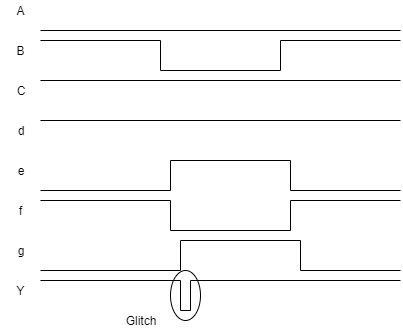
\includegraphics[width=0.6\textwidth]{figs/Ej3/glitch.jpg} % first figure itself
         \caption{Diagramas temporales del circuito en donde se aprecia el glitch en la salida.}
         \label{ej3_glitch}
\end{figure}
%
\noindent
Este glitch (indeseado) es provocado debido a los diferentes tiempos de propagaci\'on de las compuertas utilizadas, es decir existe un camino que presenta m\'as compuertas l\'ogicas que el otro por lo que se genera un momento en donde en la entrada de la compuerta or a la salida se tienen 2 ceros que no se deber\'ian encontrar, esto hace que a la salida se observe un cero por un breve instante de tiempo (el tiempo de propagación de la compuerta tomado).\\
Para evitar este tipo de glitch, lo que se hace es realizar una configuración de mayor costo, es decir, considerar un grupo extra (y por consiguiente mayor cantidad de compuertas l\'ogicas en el diseño total) que abarque los 2 unos que se hallaban adyacentes sin estar conectados mediante un grupo. Esto se puede ver en el diagrama de Karnaugh siguiente.
%
\begin{center}
    \begin{Karnaughvuit}
       \minterms{1,4,5,6}
        \maxterms{0,2,3,7}
       %\indeterminats{2,5}
       \implicantcostats{4}{6}{green}
       \implicant{1}{5}{blue}
       \implicant{4}{5}{red}
    \end{Karnaughvuit}
\end{center}
%
\noindent
De esta forma la configuraci\'on l\'ogica que cumple este circuito es la de la ecuaci\'on \ref{ej3_eq2}.
%
\begin{equation}
    \overline{A} \cdot B+\overline{B} \cdot C+\overline{A} \cdot C
    \label{ej3_eq2}
\end{equation}
%
\noindent
Por ello el circuito que cumple con dicha ecuación se muestra en la figura \ref{ej3_circuito2}.
%
\begin{figure}[H]
    \centering
        \centering
        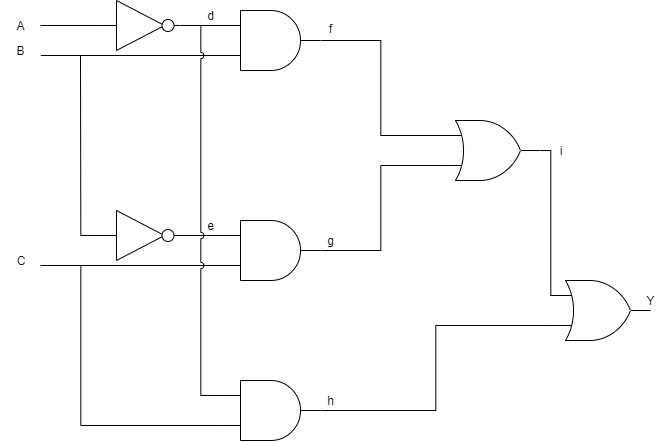
\includegraphics[width=0.6\textwidth]{figs/Ej3/circuito2.jpg} % first figure itself
         \caption{Circuito con la corrección para evitar glitches}
         \label{ej3_circuito2}
\end{figure}
%
%
\subsection{Implementaci\'on}
%
\noindent
Para comprobar esto, se realiz\'o en PCB un diseño en donde se puede trabajar tanto con un circuito como con otro a la vez, esto permite observar las diferentes salidas de cada uno para con ello poder contrastarlas y hallar diferencias entre los métodos trabajados.\\
\noindent
De esta forma, la placa PCB utilizada se puede observar en la imagen \ref{ej3_placa}.
Para la misma se utilizaron los integrados 74HC08 para las compuertas and, 74HC04 para las compuertas not y 74HC32 para las compuertas or. Los tiempos de propagación de dichas compuertas se muestran a continuación en la tabla \ref{tabla_comp_tiempos_prop}, y se pueden ver en en las hojas del fabricante \href{ http://www.ti.com/lit/ds/symlink/sn74hc08.pdf}{74HC08}, \href{http://www.ti.com/lit/ds/symlink/sn74hc04.pdf}{74HC04}, \href{http://www.ti.com/lit/ds/symlink/sn74hc32.pdf}{74HC32}.
%
\begin{table}[H]
\caption{Tabla con los tiempos de propagación de las compuertas utilizadas.}
\label{tabla_comp_tiempos_prop}
\centering
\begin{tabular}{|l||l|l|}
\hline
integrado & normal (ns) & maximo (ns) \\ \hline \hline
74HC04    & 9      & 22     \\ \hline
74HC08    & 10     & 20     \\ \hline
74HC32    & 12     & 18     \\ \hline
\end{tabular}
\end{table}
%
%
%
\begin{figure}[H]
    \centering
        \centering
        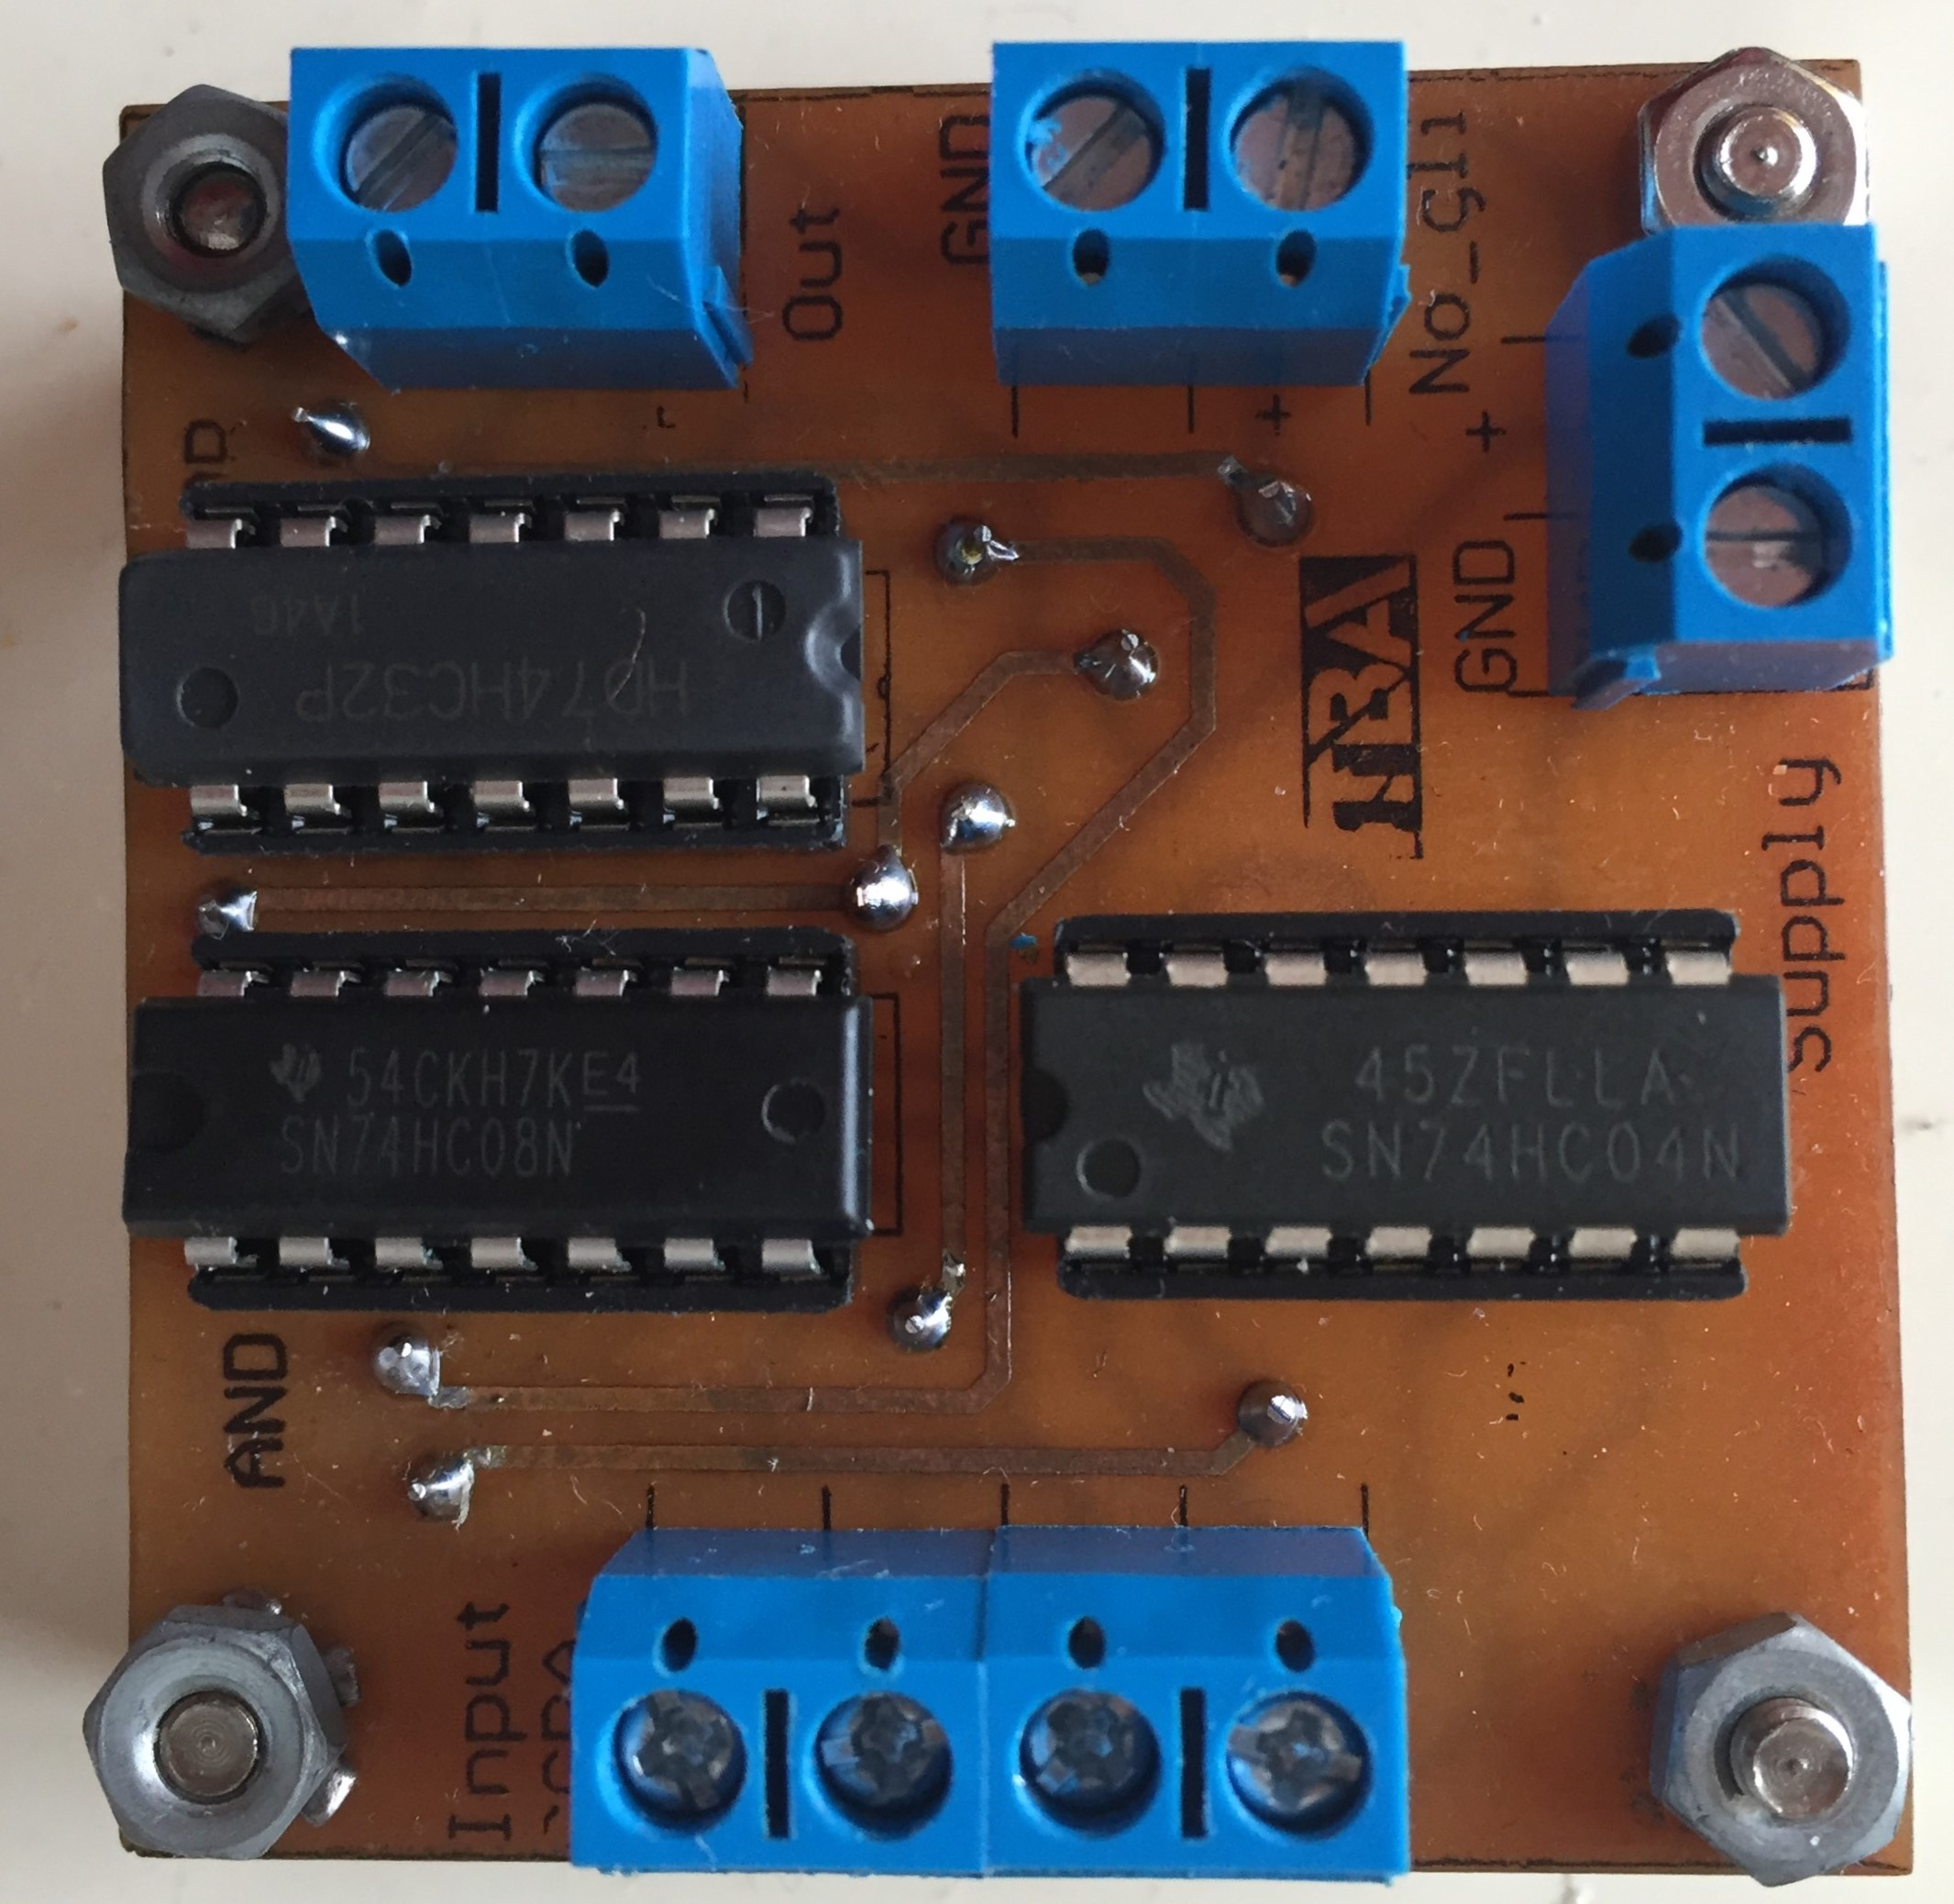
\includegraphics[width=0.6\textwidth]{figs/Ej3/Circuito_PCB.jpg} % first figure itself
         \caption{placa PCB utilizada}
         \label{ej3_placa}
\end{figure}
%
\subsection{Mediciones y Conclusiones}
\noindent
A continuación en la figura \ref{ej3_medicion} se muestra la medición del circuito a la salida del mismo, donde se superponen la salida del circuito con la configuración de menor costo y la salida del circuito con la configuración de mayor costo que soluciona el problema de los glitches, las mismas se realizaron en simultaneo en las 2 salidas del circuito destinadas a este fin, al pasar de la configuración abc=001 a abc=011, para el cambio de B se utilizó un generador de onda cuadrada con tensiones de 0V mínima y 5V máxima.\\ Cabe destacar que para poder observar el glitch es muy importante utilizar puntas x10 ya que la capacidad de las puntas x1 impide la correcta visualización de la caída en tensión.
%
\begin{figure}[H]
    \centering
        \centering
        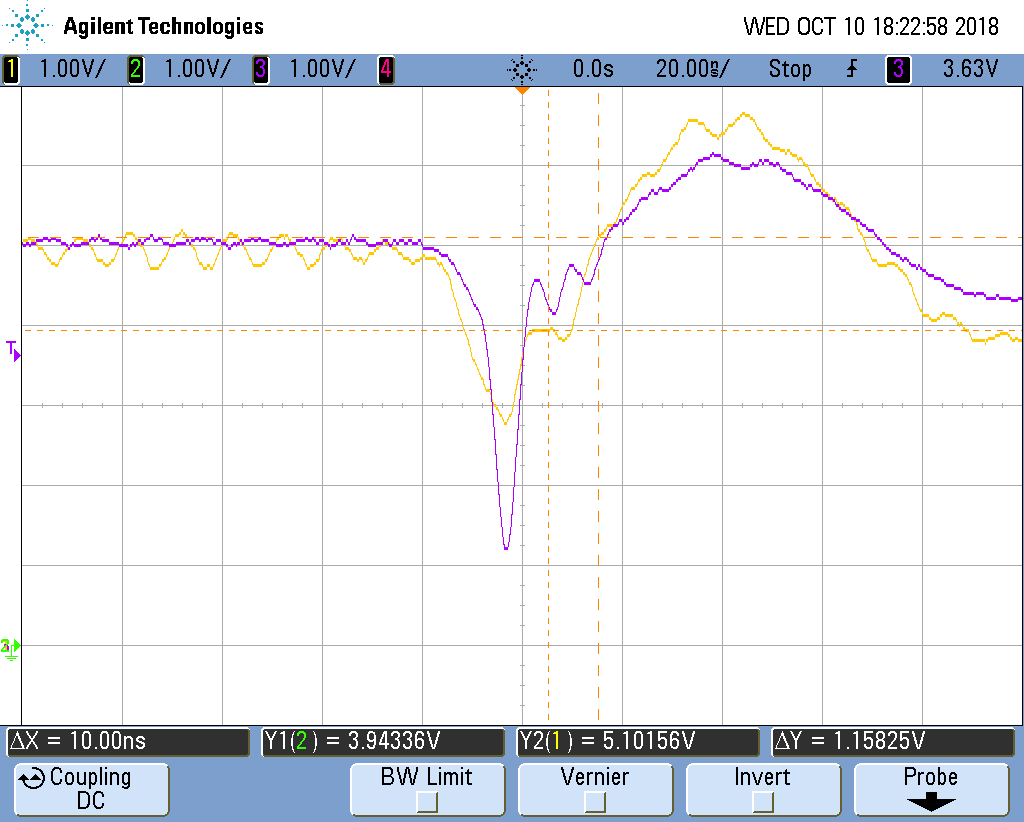
\includegraphics[width=0.6\textwidth]{figs/Ej3/x10_se_ve_glitchesito_ojo_limit_oscil.png} % first figure itself
         \caption{Medición realizada donde se aprecia el glitch a la salida.}
         \label{ej3_medicion}
\end{figure}
%
\noindent
En la imagen \ref{ej3_medicion} podemos ver las 2 salidas deseadas, la salida sin la corrección es la de color violeta, y la salida corregida corresponde a la linea de color amarillo.\\
En el osciloscopio se observa como el valor de la salida violeta cae por debajo del límite inferior tomado como High por las compuertas con tecnología CMOS (imagen \ref{ej3_cmos}), pasa por la zona de transición y llega a ser inferior que el límite superior de lo que se considera como LOW, es decir un cero lógico durante un tiempo comparable con el de las compuertas utilizadas, llegando a valer 1,2 V. Esto tiene sentido si se observa el diagrama temporal analizado anteriormente donde el tiempo del glitch se correspondía con el tiempo de propagación tomado para las compuertas. Mientras que la salida amarilla correspondiente a la salida del sistema con el glitch corregido presenta una desviación mucho menor que le permite nunca bajar lo suficiente para ser considerado por la compuerta como un 0 lógico, vemos por tanto que en la salida corregida no existe glitch mientras que en la salida violeta es decir la de menor costo si lo hay.
%
\begin{figure}[H]
    \centering
        \centering
        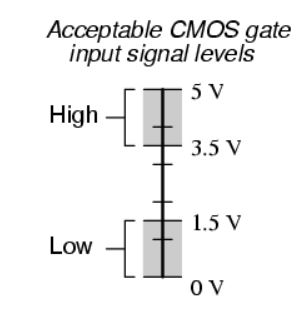
\includegraphics[width=0.4\textwidth]{figs/Ej3/cmosvoltages.JPG} % first figure itself
         \caption{Tensiones de entrada consideradas como HIGH y LOW en una compuerta con tecnología CMOS}
         \label{ej3_cmos}
\end{figure}